\chapter{Fabry-Perot cavities}
\label{sec:cavities}
In this appendix I derive the basic properties of Fabry-Perot
cavities~\cite{Fabry1892Theorie,Fabry1901New} in the plane wave approximation.
Excellent references with further detail include \cite{Siegman1990Lasers} and \cite{Fox1961Resonant}.

%\cite{Butler2004Characterization}
\subsection{Fabry-Perot field equations}

\begin{figure}
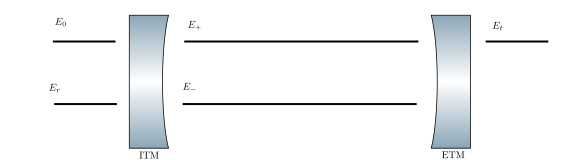
\includegraphics[]{figures/cavity.pdf}
\caption[Fabry-Perot Cavity]{\label{fig:fabry-perot}Fabry-Perot
  cavity.  When used as an arm cavity, the two mirrors are known as
  the input (ITM) and end (ETM) test masses.  Here $E_0$ indicates the
  amplitude of the incident electric field, $E_r$ the reflected field,
  $E_+$ the forward-going intra-cavity field, etc.}
\end{figure}

We begin by writing down the relationships between the fields at each
interface.  For simplicity, we treat each mirror as a single (thin)
interface.  Let $r_1$ and $t_1$ be the amplitude reflectivity and
transmissivity for the input mirror, and $r_2$ and $t_2$ describe the
output mirror.  I use the phase convention where transmission through
a mirror conveys $90^\circ$ of phase, i.e. a factor of $i$ in the
amplitude:
%
\begin{align}
E_+ &= i t_1 E_0 + r_1 E_- \\
E_- &= r_2 e^{i 2 \phi} E_+ \\
E_t &= i t_2 e^{i \phi} E_+ \\
E_r &= r_1 E_0 + i t_1 E_1
\end{align}
%
Solving these equations algebraically for $E_r$ and $E_t$ in terms of the incident field $E_0$, we find the transmission and reflectivity of the cavity:
%
\begin{align}
t_c \equiv & \frac{E_t}{E_0} = 
         \frac{-t_1 t_2 \exp i\phi}
              {1 - r_1 r_2 \exp i2\phi} \\
r_c \equiv & \frac{E_r}{E_0} = 
         \frac{r_1 - \left({r_1}^2 + {t_1}^2\right)r_2 \exp{i2\phi}}
              {1 - r_1 r_2 \exp i2\phi}
\label{eq:cavity-reflectivity}
\end{align}
%
where $\phi=(2\pi/\lambda)L$ is the phase accumulated by the field as it travels from
the first mirror to the second mirror.  This phase depends on both the
laser wavelength and the distance between the mirrors:\footnote{There is an additional contribution to the phase, the Guoy phase shift, due to geometric effects; this is described in chapter 4.  Also note that some references use the \emph{round-trip} phase rather than the \emph{one-way} phase used here.}
\begin{align}
\phi  & = \pi (\nu / \nu_0) \\
\nu_0 & = c/(2L)
\end{align}
where $\nu=c/\lambda$ is the laser frequency, $L$ is the cavity
length, and $\nu_0$ is the \emph{free spectral range}, which describes
the spacing between adjacent resonances.

\subsection{the cavity pole}
It is often useful to write the cavity reflectivity in the form of a
rational transfer function,
\begin{equation}
r_c(s) = \prod_{n=-\infty}^{\infty} \frac {s-z_n} {s-p_n}
\label{eq:rational-function}
\end{equation}
where $s=i\omega$, $\{z_n\}$ are the zeroes of $r_c(s)$, and $\{p_n\}$
are the poles.  To find the poles and zeroes, make the substitution
$\phi=-is/(2\nu_0)$ and solve for the zeroes of the numerator and
denominator of equation~\ref{eq:cavity-reflectivity} separately.  We find:
\begin{align}
p_n &= - \omega_{fsr} \left(\log\left(r_1 r_2\right) +  i n\right)  & \forall n\in \mathbb{Z}\\
z_n &= + \omega_{fsr} \left(\log\left(r_1/r_2\right) +  i n\right)  & \forall n\in \mathbb{Z}
\end{align}
where $\omega_{fsr}\equiv2\pi\nu_0$.

Because this function is periodic in $i\omega$, we can in many
circumstances regard the laser carrier as having a frequency
$\nu=0$ rather than $\nu = n\nu_0$ for some very large $n$.

\begin{figure}
\centering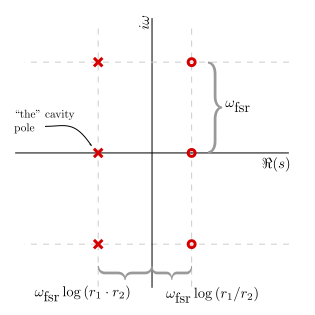
\includegraphics{figures/cavitypzmap.pdf}
\caption[Pole-zero map of Fabry-Perot cavity reflectivity]{\label{fig:cavpzmap} Pole-zero map of the cavity amplitude
  reflectivity.
  Poles are designated with $\times$ and zeros with
  $\circ$; $r_1$ is the amplitude reflectivity of the input coupler,
  and $r_2$ is the amplitude reflectivity of the output coupler.
  Losses can be lumped into $r_2$.  Notice that the free spectral
  range (angular frequency $\omega_{\textrm{fsr}}$) sets the scale of
  the entire diagram, and the function is periodic in $i\omega$: there
  is an infinite line of poles and an infinite line of zeros.  Two
  limiting cases are worth considering: (1) A critically-coupled
  cavity has $r_1=r_2$, which brings the line of zeros onto the
  imaginary axis. On resonance, $i\omega$ travels through these zeros
  and the cavity reflectivity vanishes.  This models the desired
  behavior of mode cleaner cavities. (2) A maximally over-coupled
  cavity has $r_2=1$, in which case the line of poles and line of
  zeros are equally spaced from the imaginary axis.  This models the
  LIGO arm cavities.  
  The cavity's amplitude transmission has the same poles as the
  reflectivity but no zeros.
}
\end{figure}

\subsection{phase gain}
Our interest in using Fabry-Perot cavities as the arms of a
gravitational wave detector is in having the light traverse the length
of the arm multiple times, multiplying the effect of any optical path
length perturbations caused by a GW.  We can derive the magnitude of
this \emph{phase gain} by examining how the phase of the light reflected from
the cavity changes as the intra-cavity phase $\phi$ changes, for small
variations from resonance.

Suppose $z(t)=A(t) \exp\{i \phi(t)\}$ is an arbitrary complex-valued
function with amplitude $A(t)$ and phase $\phi(t)$. By taking the
logarithm before taking the derivative, we can separate the amplitude
and phase:
%
\begin{equation}
\frac{\partial}{\partial t} \log z(t) = \left(\frac{\partial}{\partial t} \log A(t)\right) + i \left(\frac{\partial}{\partial t} \phi(t)\right)
= \frac{1}{z(t)} \frac{\partial}{\partial t} z(t)
\end{equation}
%
This gives us an expression for the rate of change of the phase of a function:
%
\begin{equation}
\frac{\partial}{\partial t} \arg z(t) = \text{Im} \frac{1}{z(t)} \frac{\partial}{\partial t} z(t)
\end{equation}

We can find the phase gain of a Fabry-Perot cavity by applying this expression to the cavity reflectivity as a function of intra-cavity phase, $r_c(\phi)$:
\begin{equation}
g_\phi = \text{Im\ } \frac{r_c'}{r_c}
\end{equation}
where $r_c'(\phi)\equiv(1/2)(\partial/\partial\phi)r_c(\phi)$; the factor of $1/2$ is to convert from round-trip phase to one-way phase.  Because the derivative of the amplitude of $r_c$ vanishes on resonance, we can simply take the magnitude of $r_c'/r_c$ rather than the imaginary part. Explicitly taking the derivative of equation~\ref{eq:cavity-reflectivity}, we find
\begin{equation}
r_c'(\phi) = \frac{1}{2}\frac{d}{d\phi} r_c(\phi) = 
-i \frac{\left(1-{r_1}^2\right) r_2 \exp 2 i \phi}
     {\left(1 - r_1 r_2 \exp 2 i \phi\right)^2}\\
\end{equation}
%
Conventionally the symbol $r_c'$ (as in \cite{LigoFreqResponse97}) indicates the magnitude of this expression at resonance ($\phi=0$):
\begin{equation}
r_c' = 
 \frac{\left(1-{r_1}^2\right) r_2 }
     {\left(1 - r_1 r_2 \right)^2}
\end{equation}

Another way to calculate the phase gain is to use the rational transfer function expression, equation~\ref{eq:rational-function}.  To model the situation near resonance, we need only consider the nearest pole and zero:
\[
r_c(s) \approx \frac{s - z_0}{s - p_0}
 = \frac{s - \omega_{fsr}\log \left(r_1 / r_2\right)}
        {s + \omega_{fsr}\log \left(r_1 \cdot r_2\right)}
\]
Recall that the phase at frequency $\omega$ imparted by a pole at
frequency $\omega_c$ is $\arctan\left(-\omega/\omega_c\right)$; a zero
at the same frequency subtracts this same phase.  For a maximally
over-coupled cavity (i.e. with $r_2 = 1$), the cavity pole and cavity
zero are equal and opposite, so contribute equal phase ($\arctan$ is
odd).  Use $\omega = 2\nu_0\phi$ to express the detuning phase $\phi$
as an equivalent detuning frequency.

Changing the one-way phase of the arm by $\phi$ results in a phase 
change of
\begin{equation}
\phi_r   = 2 \tan^{-1} \left( 2 \nu_0 \frac{\phi}{\omega_c} \right)
%   = 2 \tan^{-1} \left( \frac{2}{\pi}\mathcal{F}\phi\right)
\end{equation}
where $\omega_c\equiv2\pi f_c$ is the cavity pole and $\mathcal{F}=(1/2)(\nu_0/f_c)$ is the cavity finesse (which will be introduced in section~\ref{sec:finesse}).  Taking the derivative, we find the phase gain:
\begin{equation}
g_\phi =  \frac{1}{2} \frac{d \phi_r}{d \phi} 
= \frac{2 \nu_0}{\omega_c} \left[1 + \left(\frac{2 \nu_0 \phi}{\omega_c}\right)^2 \right]^{-1} 
= \frac{2 \mathcal{F}}{\pi} \left[1 + \left(\frac{\omega}{\omega_c}\right)^2 \right]^{-1} 
\end{equation}
The phase gain on resonance is $2 \nu_0 / \omega_c = 2\mathcal{F}/\pi \approx 140$. This phase gain decreases as we detune the cavity further from resonance, but it is not seriously diminished until the cavity detuning approaches the cavity pole.

\subsection{intra-cavity power buildup}

The power buildup in the cavity is given by 
\begin{equation}
\frac{P_+}{P_{IN}} = \frac{|E_+|^2}{|E_0|^2} = \frac{ T_1}{1 - 2 r_1 r_2 \cos 2\phi+\left(r_1 r_2\right)^2 }
\end{equation} 
which may be re-written (using the identity $\cos2\phi = 1 -
2\sin^2\phi$) as
\begin{equation}
\label{cavity_buildup_eq}
\frac{P_+}{P_{IN}} = \frac{g^2}{1 + F \sin^2 \phi} 
\text{  with  } F = \frac{4 r_1 r_2}{(1 - r_1 r_2)^2}
\text{  and  } g = \frac{t_1}{1-r_1 r_2}
\end{equation} 
where $F$ is the \emph{coefficient of finesse} and $g$ is the
\emph{amplitude gain}.

The form of this expression is often referred to in the literature as
an Airy function, though it is distinct from the well-known special
function of the same name.  Making the small angle approximation
$\sin\phi\approx\phi$ we see that each resonance is locally Lorentzian.

\subsection{finesse ($\mathcal{F}$)}
\label{sec:finesse}
The tightness of the resonance is quantified as the
\emph{finesse} ($\mathcal{F}$), which is defined as the ratio of the
cavity free spectral range to the full-width-half-max of the
resonance,
\begin{equation}
\mathcal{F} \equiv \frac{\nu_0}{\nu_{\mathrm{FWHM}}}
= \frac{1}{2}\frac{\nu_0}{f_c}
\end{equation}
%
where the FWHM is given by twice the cavity pole ($f_c$).  The finesse is related to the coefficient of finesse ($F$) by
%
\begin{equation}
\mathcal{F} = \frac{\pi}{2} \frac{1}{{\sqrt{\arcsin (1/F)}}} \approx \frac{\pi}{2}\sqrt{F}
\end{equation}where the approximation holds for high-finesse cavities.

The finesse ($\mathcal{F}$) of an optical cavity is analogous to
the quality factor (Q) of an oscillator. The Q factor is the ratio
of the frequency of an oscillator to its full-width-half-max bandwidth;
to compute finesse, the free spectral range (spacing between resonances)
is used instead of the oscillator frequency.

\begin{figure}
\begin{centering}
\includegraphics{figures/finesses}
\end{centering}
\caption[Cavity buildup versus detuning]{Power transmission coefficients for three critically-coupled cavities.}
\end{figure}

\subsection{Impedance matching}

From the point of view of a beam incident upon a cavity, the cavity is
either under coupled, critically coupled, or over coupled. This
coupling is determined by the comparison of the transmissivity of the
input coupler compared to all other losses in the system. For a
two-mirror, lossless cavity, the cavity is under coupled if $t_1 <
t_2$, critically coupled if $t_1 = t_2$, and over coupled if $t_1 >
t_2$.

%For a discussion of impedance in acoustic context, see \cite{Blackstock2000Fundamentals}.

\begin{figure}
\subfloat[Critically coupled cavity. Note that $r=0$ on resonance. Cavities
of this type are used as filter cavities.]{\includegraphics{figures/circles-critically-coupled}}\hfill \subfloat[Maximally over-coupled cavity. Note that $r=-1$ on resonance. Cavities
of this type are used for the LIGO arms.]{\includegraphics{figures/circles-over-coupled}}\caption[Cavity amplitude reflectivity plotted in the complex plane]{Reflection coefficients for two cavities, plotted on the complex plane,
over a free spectral range $0\leq\phi<\pi$. The x axis represents
the real part, and the y axis the imaginary part of the cavity reflection
coefficient. The dots are spaced with uniform $\Delta\phi$. They
appear more closely spaced when the phase of the cavity reflectivity
changes slowly; they appear sparsely spaced where the reflected phase
changes quickly, as the cavity goes through resonance.}
\end{figure}

\subsubsection{Critically-coupled cavities}

Maximum power is transfered into a critically coupled cavity; no power
is reflected. In this case, the prompt reflection from the input coupler
is exactly canceled by an equal-amplitude, opposite-phase leakage
beam from the field inside the cavity. Because an (ideal) critically
coupled resonator is perfectly transmissive for light at the resonant
frequency, they are used as filter cavities.

The transmission of power through a filter cavity may be found by
multiplying equation \ref{eq:powerbuildup} by the output coupler
power transmissivity $T={t_{1}}^{2}={t_{2}}^{2}$: 
\begin{equation}
T_{c}=\frac{1}{1+F\sin^{2}\phi}=\begin{cases}
1 & \text{at resonance (maximum transmission)}\\
1/(1+F) & \text{at anti-resonance (minimum transmission)}
\end{cases}
\end{equation}
where we see that the (coefficient of) finesse quantifies the attenuation
of non-resonant modes (in addition to the width of the resonance).

The power buildup inside a critically-coupled two-mirror cavity is
simply the inverse of the mirror transmission:
\[
g^{2}=\left(\frac{t_{1}}{1-r_{1}r_{2}}\right)^{2}=\frac{t^{2}}{\left(1-r^{2}\right)^{2}}=\frac{1}{T}
\]
This can also be seen from a very simple argument: if the power emerging
from the output coupler is equal to $P_{IN}$, then the power inside
the cavity must be $P_{IN}/T$.


\subsubsection{Over-coupled cavities}

The LIGO arms are strongly over-coupled cavities. A lossless maximally over-coupled
cavity (i.e. with $t_{2}=0$) acts as a perfect reflector. 

For high-finesse, highly-overcoupled cavities, the cavity power buildup
$g^{2}$ is approximately equal to the square root of the coefficient
of finesse, or $(2/\pi)$ times the finesse:
\begin{equation}
g^{2}\approx\sqrt{F}\approx\frac{2}{\pi}\mathcal{F}
\end{equation}
This can be seen by setting $r_{2}=1$ and using $\sqrt{x}\approx1+(x-1)/2$
for $x\approx1$:
\begin{equation}
g^{2}\bigg|_{r_{2}\to1}=\frac{1-r_{1}^{2}}{\left(1-r_{1}\right)^{2}}=\frac{1+r_{1}}{1-r_{1}}\approx\frac{2\sqrt{r_{1}}}{1-r_{1}}=\sqrt{F}\bigg|_{r_{2\to1}}
\end{equation}
%
%
Another useful approximation is:
\[
g^{2}\approx\frac{4}{T_{1}}
\]
